\section{CORRELATION}
As stated before, we are interested in the correlation between Interest Rates, Consumer Price Index and Gross Domestic Product in order to understand if the current economic theory of increasing interest rate to control inflation and maintaining a healthy economy is true. As a first step, to this analysis we conduct a correlation analysis between the three variables. In order to achieve more reliable results without making any assumptions about the distribution of the data, we calculate the correlation coefficients using bootstrapping.

\subsection*{Statistical Background}
There are many ways to measure the correlation between two variables. The most common method is the Pearson correlation coefficient which is a measure of linear correlation between two variable $X$ and $Y$.
\begin{equation*}
    \rho_{X,Y} = \frac{cov(X,Y)}{\sigma_X \sigma_Y} = \frac{E[(X-\mu_X)(Y-\mu_Y)]}{\sigma_X \sigma_Y}
\end{equation*}
The Pearson correlation coefficient is a value between -1 and 1 where 1 means that the two variables are perfectly correlated, 0 means that there is no correlation and -1 means that the two variables are perfectly negative-correlated.

More options are available to measure the correlation between two variable. For example, the Spearman's rank correlation coefficient is a measure of monotonic correlation, whether linear or not. It is equivalent to the Pearson correlation coefficient of the rank variables where the rank of a variable is the position the variable would have if the data were sorted in ascending order.
\begin{align*}
    \rho_{X,Y} & = 1 - \frac{6 \sum d_i^2}{n(n^2-1)} \\
    d_i        & = rank(X_i) - rank(Y_i)
\end{align*}
where $d_i$ is the difference between the ranks of the two variables for the $i$-th observation.

It is important to remember that more complex relationships can exist between variables that neither the Pearson nor the Spearman correlation coefficient can capture (e.g. quadratic relationships).

Another measure of rank correlation is the Kendall's tau coefficient which is a measure of the correspondence between the rankings of two variables:
\begin{align*}
    \tau = \frac{P-Q}{\frac{1}{2}n(n-1)} \\
\end{align*}
where $P$ is the number of concordant pairs and $Q$ is the number of discordant pairs. A pair of observations $(x_{i},y_{i})$ and $( x_j , y_j) $ is said to be concordant if the sort order of $( x_i , x_j )$ and $( y_i , y_j )$ agrees: that is, if either both  $x_{i}>x_{j}$ and  $y_{i}>y_{j}$ or both $\displaystyle x_{i}<x_{j}$ and $y_{i}<y_{j}$ holds.

Because they deal with with rank variables instead of raw data, the Spearman and Kendall coefficients are less sensitive to outliers than the Pearson coefficient.

\subsection*{Results}
In figure \ref{fig:correlation_italy} we show the correlation between Interest Rates, Consumer Price Index and Gross Domestic Product for Italy. The correlation coefficients are calculated using bootstrapping with 1000 repetitions. The confidence intervals are calculated using the percentile method with a confidence level of 95\%.
As we can see in \ref{fig:correlation_italy}, the correlation between Interest Rates and Consumer Price Index is strongly negative, while the correlation between Interest Rates and Gross Domestic Product is weakly negative as we expected.

\begin{figure}[H]
    \centering
    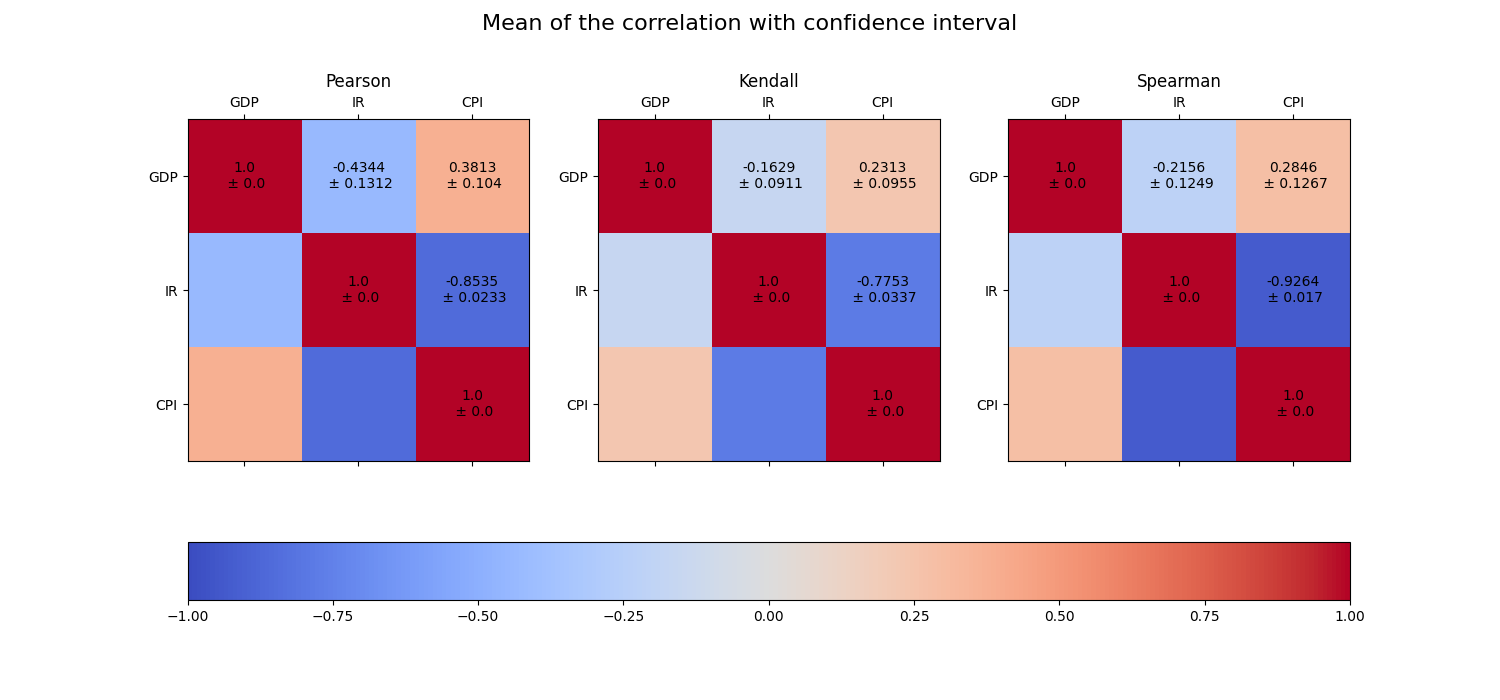
\includegraphics[width=\linewidth]{imgs/italy_correlation.png}
    \caption{Correlation between Interest Rates, Consumer Price Index and Gross Domestic Product of Italy}
    \label{fig:correlation_italy}
\end{figure}

For other countries, for example the United States (figure \ref{fig:correlation_us}), both the correlation between Interest Rates and Consumer Price Index and the correlation between Interest Rates and Gross Domestic Product are stronger than for Italy. This could be caused by the strong and self sufficient economy of the USA: being less dependant on other conditions like international trading, other countries crisis or slow growth, and being the central economic power of the world, the monetary policies of the Federal Reserve (the american Central Bank) have more impact on the internal economy.

\begin{figure}[H]
    \centering
    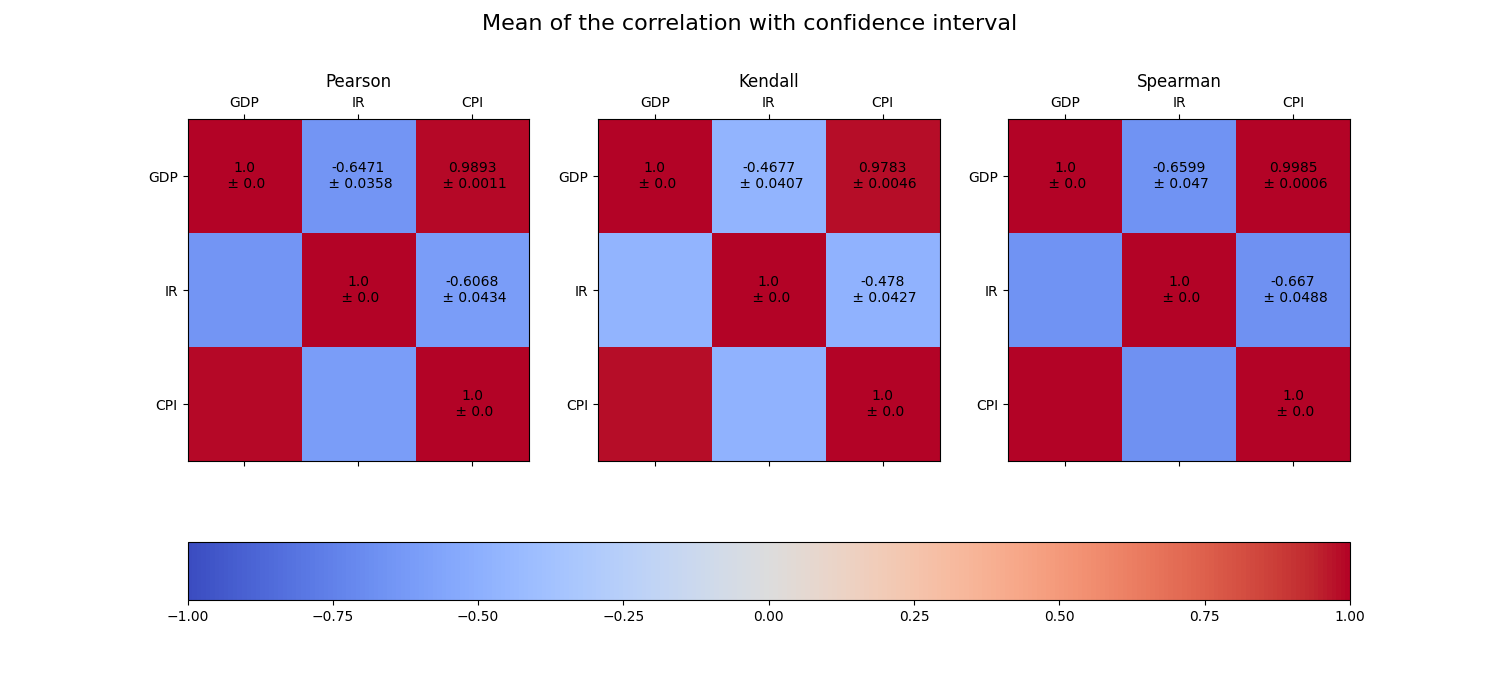
\includegraphics[width=\linewidth]{imgs/usa_correlation.png}
    \caption{Correlation between Interest Rates, Consumer Price Index and Gross Domestic Product of the United States of America}
    \label{fig:correlation_us}
\end{figure}

We also analyze the overall relationships by putting together the data for all countries in figure \ref{fig:correlation_global}. We can observe that the correlation between Interest Rates and Consumer Prince Index remains negative albeit weaker than for the individual countries above while the correlation between Interest Rates and Gross Domestic Product is very weakly positive. This could be due to the fact that economies have different conditions and responses to economic stimulus. Our analysis is also simplified and does not consider steps of increases, putting as the same an inflation of 3\%, which is good according to the current economic theory, and 20\%, which is too high and dangerous.

\begin{figure}[H]
    \centering
    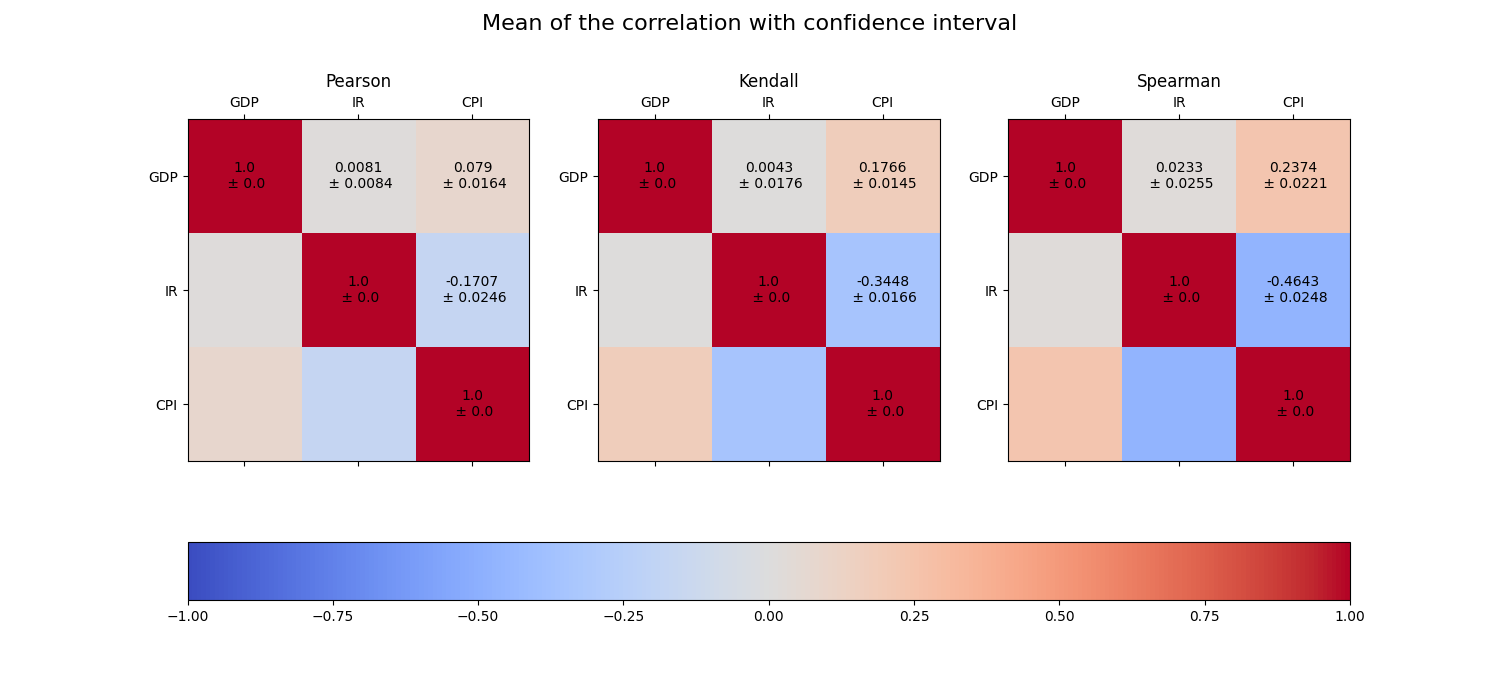
\includegraphics[width=\linewidth]{imgs/all_countries_correlation.png}
    \caption{Correlation between Interest Rates, Consumer Price Index and Gross Domestic Product of all economies studied combined}
    \label{fig:correlation_global}
\end{figure}

This first analysis shows us that the correlation between the three variable is not entirely as we expected. This could be due to the fact that the relationship between the variables is very complex and cannot be captured by simple linear or monotonic correlation coefficients.
